% !TeX spellcheck = ru_RU
% !TEX root = vkr.tex

\section{Эксперимент}

Целями следующих экспериментов является выявление возможной зависимости пропускной способности рантайма от взаимодействия воркеров с глобальной очередью.

\subsection{Условия эксперимента}

\begin{itemize}
    \item Исследования проводились на системе YADRO VEGMAN Rx20 G2\footnote{\href{https://yadro.com/ru/vegman/rx20g2/specs}{Описание} системы YADRO VEGMAN Rx20 G2}.
    \item Бенчмарк был запущен с значением \verb|nice| равным минус двадцати.
    \item Исполнение было рекомендовано на одной NUMA единице с помощью \verb|taskset|.
\end{itemize}

Машина для измерение производительности была любезно предоставлена командой \verb|TATLIN.BACKUP| и находилась удаленно, в связи с чем на ней было невозможно отключение сети.

criterion был конфигурирован следующим образом:

\begin{itemize}
    \item пять секунд прогрева.
    \item сорок семплов для каждого измерения.
    \item линеаризация в качестве способа семплирования.
\end{itemize}

\subsection{Ход исследования}

Для проверки гипотезы об ограничении производительности ресурсами одного рантайма, были произведены измерения пропускной способности системы, состоящей из нескольких рантаймов приведенной приведенные на графике \ref{fig:tatlin:multi_rt:eval}. Задачи производились потоками воркеров --- добавлялись в глобальную очередь при переполнении пачками. Каждое измерение использовало одинаковое количество системных потоков разделяемое между рантаймами.

\begin{figure}[H]
    \begin{center}
        \makebox[\textwidth]{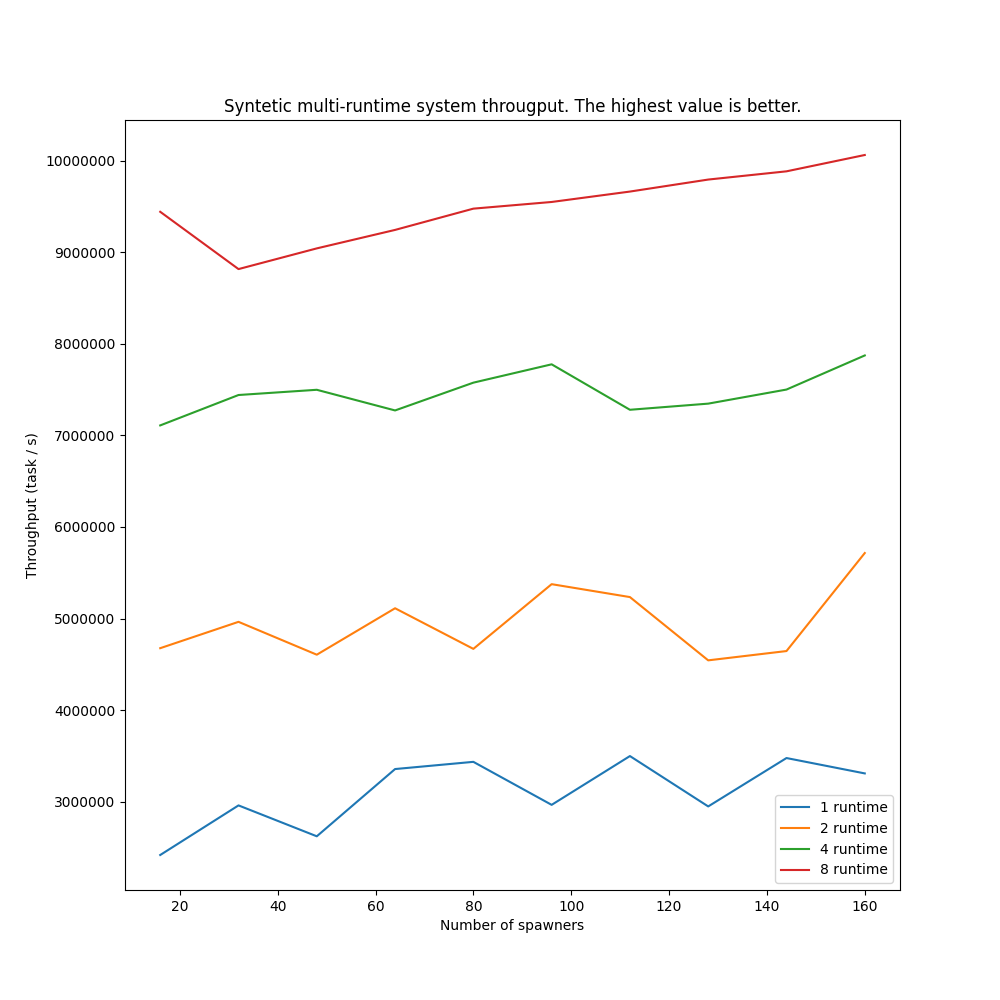
\includegraphics[scale=0.40]{pictures/multi_rt_eval.png}}
    \end{center}

    \caption{Производительность системы при использовании нескольких рантаймов}
    \label{fig:tatlin:multi_rt:eval}
\end{figure}

Из рисунка заметным становится увеличение производительности пропорционально количеству рантаймов.

\subsection{Вывод}

Глобальная очередь может накладывать ограничение на производительность всего рантайма.

\begin{itemize}
    \item При дубликации ресурсов (OwnedQueue, InjectQueue) наблюдается увеличение пропускной способности.
    \item Существуют ресурсы tokio разделяемые между различными инстансами, например атомарная переменная генерирующая индентификатор задач.
\end{itemize}
